\documentclass[boxes]{homework}

% This is a slightly-more-than-minimal document that uses the homework class.
% See the README at http://git.io/vZWL0 for complete documentation.

\name{傅申 PB20000051}        % Replace (Your Name) with your name.
\term{2022 秋}     % Replace (Current Term) with the current term.
\course{算法基础}    % Replace (Course Name) with the course name.
\hwnum{11}          % Replace (Number) with the number of the homework.
\hwname{作业}
\problemname{}
\solutionname{解:}

% Load any other packages you need here.
\usepackage[
    a4paper,
    top = 2.54cm,
    bottom = 2.54cm,
    left = 1.91cm,
    right = 1.91cm,
    includeheadfoot
]{geometry}
\fancyfootoffset{0pt} % make fancyhdr work properly
\usepackage{ctex}
\usepackage{floatrow}
\usepackage{tikz}
\tikzset{
    every node/.style={circle, draw, minimum size=1.5em, inner sep=0.2em},
    marked/.style={fill=black!20},
}

\begin{document}
%%%% Problem 19.2-1 %%%%
\problemchap{19}
\problempart{2}
\problemnumber{1}
\begin{problem}
给出图 19--4 (m) 中的斐波那契堆调用 {\sc Fib-Heap-Extract-Min} 后得到的斐波那契
堆.
\end{problem}
\begin{solution}
    如下
    \begin{center}
        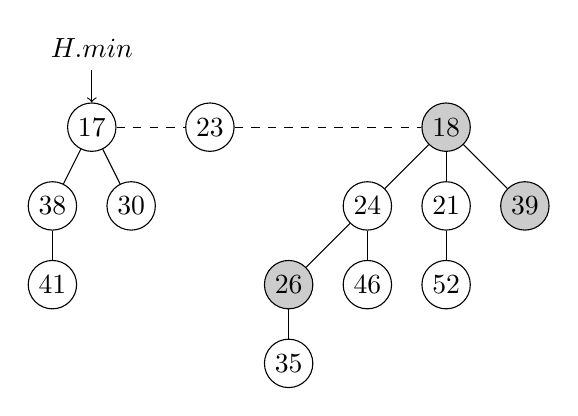
\begin{tikzpicture}
            % Heap 1
            \node (1)   at (0.5, 3) {17};
            \node (11)  at (0, 2)   {38};
            \node (111) at (0, 1)   {41};
            \node (12)  at (1, 2)   {30};
            % Heap 2
            \node (2)  at (2, 3) {23};
            % Heap 3
            \node[marked] (3)    at (5, 3) {18};
            \node         (31)   at (4, 2) {24};
            \node[marked] (311)  at (3, 1) {26};
            \node         (3111) at (3, 0) {35};
            \node         (312)  at (4, 1) {46};
            \node         (32)   at (5, 2) {21};
            \node         (321)  at (5, 1) {52};
            \node[marked] (33)   at (6, 2) {39};
            % In-heap paths
            \path[-]
            (1)  edge (11)
            (1)  edge (12)
            (11) edge (111)
            (3)  edge (31)
            (31) edge (311)
            (31) edge (312)
            (3)  edge (32)
            (32) edge (321)
            (3)  edge (33)
            (311) edge (3111)
            ;
            % Between-root paths
            \path[-, dashed]
            (1) edge (2)
            (2) edge (3)
            ;
            % Fibonacci heap minimum
            \node[draw=none, rectangle] (min) at (0.5, 4) {$H.min$};
            \draw[->] (min) -- (1);
        \end{tikzpicture}
    \end{center}
\end{solution}

%%%% Problem 19.3-1 %%%%
\problempart{3}
\problemnumber{1}
\begin{problem}
假定斐波那契堆中的一个根 $x$ 被标记了. 解释 $x$ 是如何成为一个被标记的根的. 试说
明 $x$ 是否被标记对分析并没有影响, 即使它不是一个先被链接到另一个结点, 后又丢失
了一个孩子的根.
\end{problem}
\begin{solution}
    $x$ 之前是 $H.min$ 的一个被标记的子结点, 随后执行了
    {\sc Fib-Heap-Extract-Min} 操作使得 $x$ 成为了一个被标记的根.

    一个结点是否被标记只会在 {\sc Cascading-Cut} 的第 3 行中被测试, 但是根结点在
    其第 2 行测试中就会返回, 因此 $x$ 是否被标记对实际代价并没有影响. 虽然在摊还
    分析中 $x$ 被标记会使得势函数的值大于实际需要的值, 但是多出来的值并不影响
    {\sc Fib-Heap-Decrease-Key} 的摊还代价.
\end{solution}

%%%% Problem 19.4-2 %%%%
\problempart{4}
\problemnumber{2}
\begin{problem}
假定对级联切断操作进行推广, 对于某个整数常数 $k$, 只要一个结点失去了它的第 $k$
个孩子, 就将其从它的父结点上剪切掉 (19.3 节中为 $k = 2$ 的情形). $k$ 取什么值时,
有 $D(n) = O(\lg n)$.
\end{problem}
\begin{solution}
    推广后, 引理 19.1 可重写为: 设 $x$ 是堆中的任意结点, 并假定 $x.degree = d$.
    设 $y_{1}, y_{2}, \ldots, y_{d}$ 表示以链入先后顺序排序的 $x$ 的孩子结点, 则
    对 $k - 1 \geqslant i \geqslant 1$, 有
    $y_{i}.degree \geqslant 0$; 对 $d \geqslant j \geqslant k$, 有
    $y_{j}.degree \geqslant j - k$.

    定义数列 $F$ 为
    \[
        F_{m} =
        \begin{cases}
            0                     & \mathbf{if} \quad m = 0                     \\
            1                     & \mathbf{if} \quad k \geqslant m \geqslant 1 \\
            F_{m - 1} + F_{m - k} & \mathbf{if} \quad m \geqslant k + 1
        \end{cases}
        .
    \]
    则对于所有的 $m \geqslant 0$, 有
    \[
        F_{m + k} = 1 + \sum_{i = 0}^{m} F_{i}
        .
    \]
    且若记 $\alpha$ 为方程 $x^{k} = x^{k - 1} + 1$ 的正根, 则对于所有整数
    $m \geqslant 0$, 有 $F_{m + k} \geqslant \alpha^{m}$.

    设 $s_{m}$ 表示堆中度数为 $m$ 的任意结点的最小可能 size. 平凡地, $s_{0}=1$,
    $s_{1} = 2$, $\ldots$, $s_{k - 1} = k$. $s_{m}$ 随着 $m$ 单调递增. 有
    $\operatorname{size}(x) \geqslant s_{d}$. 考虑 $d \geqslant k$ 的情况, 有
    \[
        \operatorname{size}(x) \geqslant s_{d} \geqslant k +
        \sum_{i = k}^{d} s_{y_{i}.degree} \geqslant k + \sum_{i = k}^{d}
        s_{i - k}
        .
    \]
    可以对 $d$ 归纳证明出 $s_{d} \geqslant F_{d + k} \geqslant \alpha^{d}$. 因
    此, 对任意结点 $x$ 都有 $n \geqslant \operatorname{size}(x) \geqslant
        \alpha^{d}$, 所以任意结点的最大度数 $D(n)$ 为 $O(\lg n)$. 上面的论证对所
    有正整数 $k$ 都成立.
\end{solution}

%%%% Problem 21.2-2 %%%%
\problemchap{21}
\problempart{2}
\problemnumber{2}
\begin{problem}
给出下面程序的结果数据结构, 并回答该程序中 {\sc Find-Set} 操作返回的答案. 这里使
用加权合并启发式策略的链表表示.

\RestyleAlgo{plain}
\begin{algorithm}[H]
    \For{$i = 1$ \textbf{to} 16}{
        $\operatorname{MAKE-SET}(x_{i})$\;
    }
    \For{$i = 1$ \textbf{to} 15 \textbf{by} 2}{
        $\operatorname{UNION}(x_{i}, x_{i + 1})$\;
    }
    \For{$i = 1$ \textbf{to} 13 \textbf{by} 4}{
        $\operatorname{UNION}(x_{i}, x_{i + 2})$\;
    }
    $\operatorname{UNION}(x_{1}, x_{5})$\;
    $\operatorname{UNION}(x_{11}, x_{13})$\;
    $\operatorname{UNION}(x_{1}, x_{10})$\;
    $\operatorname{FIND-SET}(x_{2})$\;
    $\operatorname{FIND-SET}(x_{9})$\;
\end{algorithm}
假定如果包含 $x_{i}$ 和 $x_{j}$ 的集合有相同的大小, 则
$\operatorname{UNION}(x_{i}, x_{j})$ 表示将 $x_{j}$ 所在的表链接到 $x_{i}$ 所在
的表后.
\end{problem}
\begin{solution}
    执行完第 1 行的循环后, 建立了 16 个只含有一个成员 $x_{i}$ 的集合.

    执行完第 3 行的循环后, 共有 8 个集合, 分别为
    \[
        \{x_{1} \to x_{2}\},
        \{x_{3} \to x_{4}\},
        \{x_{5} \to x_{6}\},
        \{x_{7} \to x_{8}\},
        \{x_{9} \to x_{10}\},
        \{x_{11} \to x_{12}\},
        \{x_{13} \to x_{14}\},
        \{x_{15} \to x_{16}\}.
    \]
    执行完第 5 行的循环后, 共有 4 个集合, 分别为
    \[
        \{x_{1} \to x_{2} \to x_{3} \to x_{4}\},
        \{x_{5} \to x_{6} \to x_{7} \to x_{8}\},
        \{x_{9} \to x_{10} \to x_{11} \to x_{12}\},
        \{x_{13} \to x_{14} \to x_{15} \to x_{16}\}.
    \]
    第 7 行的 {\sc Union} 操作结束后, 共有 3 个集合, 分别为
    \[
        \{x_{1} \to x_{2} \to x_{3} \to x_{4} \to x_{5} \to x_{6} \to x_{7}
        \to x_{8}\},
        \{x_{9} \to x_{10} \to x_{11} \to x_{12}\},
        \{x_{13} \to x_{14} \to x_{15} \to x_{16}\}.
    \]
    第 8 行的 {\sc Union} 操作结束后, 共有 2 个集合, 分别为
    \[
        \{x_{1} \to x_{2} \to x_{3} \to x_{4} \to x_{5} \to x_{6} \to x_{7}
        \to x_{8}\},
        \{x_{9} \to x_{10} \to x_{11} \to x_{12} \to x_{13} \to x_{14} \to
        x_{15} \to x_{16}\}.
    \]
    第 9 行的 {\sc Union} 操作结束后, 共有 1 个集合, 为
    \[
        \{x_{1} \to x_{2} \to x_{3} \to x_{4} \to x_{5} \to x_{6} \to x_{7}
        \to x_{8} \to x_{9} \to x_{10} \to x_{11} \to x_{12} \to x_{13}
        \to x_{14} \to x_{15} \to x_{16}\}.
    \]
    第 10 行的 $\operatorname{FIND-SET}(x_{2})$ 和第 11 行的
    $\operatorname{FIND-SET}(x_{9})$ 均返回指向 $x_{1}$ 的指针.
\end{solution}

%%%% Problem 21.3-3 %%%%
\problempart{3}
\problemnumber{3}
\begin{problem}
给出一个包含 $m$ 个 {\sc Make-Set}, {\sc Union} 和 {\sc Find-Set} 操作的序列 (其
中有 $n$ 个是 {\sc Make-Set} 操作), 当仅使用按秩合并时, 需要 $\Omega(m\lg n)$ 时
间.
\end{problem}
\begin{solution}
    假定 $m \gg n$. 先执行 $n$ 个 {\sc Make-Set} 操作, 创建 $n$ 个只有一个成员的
    集合. 然后执行 $2^{\lfloor \lg n \rfloor} - 1$ 次 {\sc Union} 操作, 将
    $2^{\lfloor \lg n \rfloor}$ 个结点合并为深度为 $\lfloor \lg n \rfloor$ 的树,
    其中每次都是选择两棵结点数为 $2^{k}$ 的树合并为一棵结点数为 $2^{k+1}$ 的树,
    这样树中就有且只有一个结点的深度为 $k + 1$, 操作的参数均为树根. 最后执行
    $m - n - 2^{\lfloor \lg n \rfloor} + 1$ 次 {\sc Find-Set} 操作, 每次执行的参
    数均为深度最高的结点.

    {\sc Make-Set} 需要 $\Omega(n)$ 的时间, {\sc Union} 需要 $\Omega(n)$ 的时间,
    {\sc Find-Set} 需要 $\Omega((m - 2n)\lg n)$ 的时间, 因为 $m \gg n$, 所以总时
    间为 $\Omega(m\lg n)$.
\end{solution}

\end{document}
